\documentclass[letter]{article}

%% Language and font encodings
\usepackage[english]{babel}
\usepackage[utf8x]{inputenc}
\usepackage[T1]{fontenc}
\usepackage{enumitem}
\usepackage{fancyhdr}
\pagestyle{fancy}

%% Useful packages
\usepackage{amsmath, amsthm, amssymb}
\usepackage{graphicx}
\newtheoremstyle{case}{}{}{}{}{}{:}{ }{}
\theoremstyle{case}
\newtheorem{case}{}


\title{HW Template}
\author{Nicholas Silva Tee}
\lhead{Homework 4 Report}



\begin{document}

\subsection*{Part 1}
This is a high level description of what why code does. \\
\textbf{1)} Create lists M, alpha and w which will contain the classifiers, confidence factors, and weights. \\
\textbf{2)} Using the training data points and the weight list create a linear classifier using the same process as we had done in HW2. Then append it to M \\
\textbf{3)} Using the classifier that we just made, test it using the training data and keep track of all the errors in the predictions.\\
\textbf{4)} Using the errors calculate the error rate, confidence factor and weight factors. Also append the confidence factor to the alpha list\\
\textbf{5)} Update the weight list with the weight factors accordingly.\\
\textbf{6)} If the error rate is less than 0.5 then jump back to step 1
\newpage
\subsection*{Part 2}
------------------------------- \\
Iteration:  1 \\
Error: 0.1875 \\
Alpha: 0.7332\\
Factor to increase weights = 2.67 \\
Factor to decrease weights = 0.62 \\
------------------------------- \\
-------------------------------\\
Iteration:  2 \\
Error: 0.2718 \\
Alpha: 0.4928 \\
Factor to increase weights = 1.84 \\
Factor to decrease weights = 0.69\\
-------------------------------\\
-------------------------------\\
Iteration:  3\\
Error: 0.625\\
Alpha: -0.2554\\
Factor to increase weights = 0.8\\
Factor to decrease weights = 1.33\\
-------------------------------\\
-------------------------------\\
Iteration:  4\\
Error: 0.9526\\
Alpha: -1.5006\\
Factor to increase weights = 0.52\\
Factor to decrease weights = 10.56\\
-------------------------------\\
-------------------------------\\
Iteration:  5\\
Error: 0.9977\\
Alpha: -3.0385\\
Factor to increase weights = 0.5\\
Factor to decrease weights = 218.37\\
-------------------------------\\
Testing: \\
False positives: 3\\
False negatives: 15\\
Error rate: 22.5\\

\subsection*{Part 3}
Basic linear classifier error rate: 18.75\%\\
\\
error rate of boosted version:\\
\textbf{T = 1:} 18.75\% \\
\textbf{T = 2:} 17.5\% \\
\textbf{T = 3:} 20\% \\
\textbf{T = 4:} 18.75\% \\
\textbf{T = 5:} 22.5\% \\

\begin{figure}[h!]
	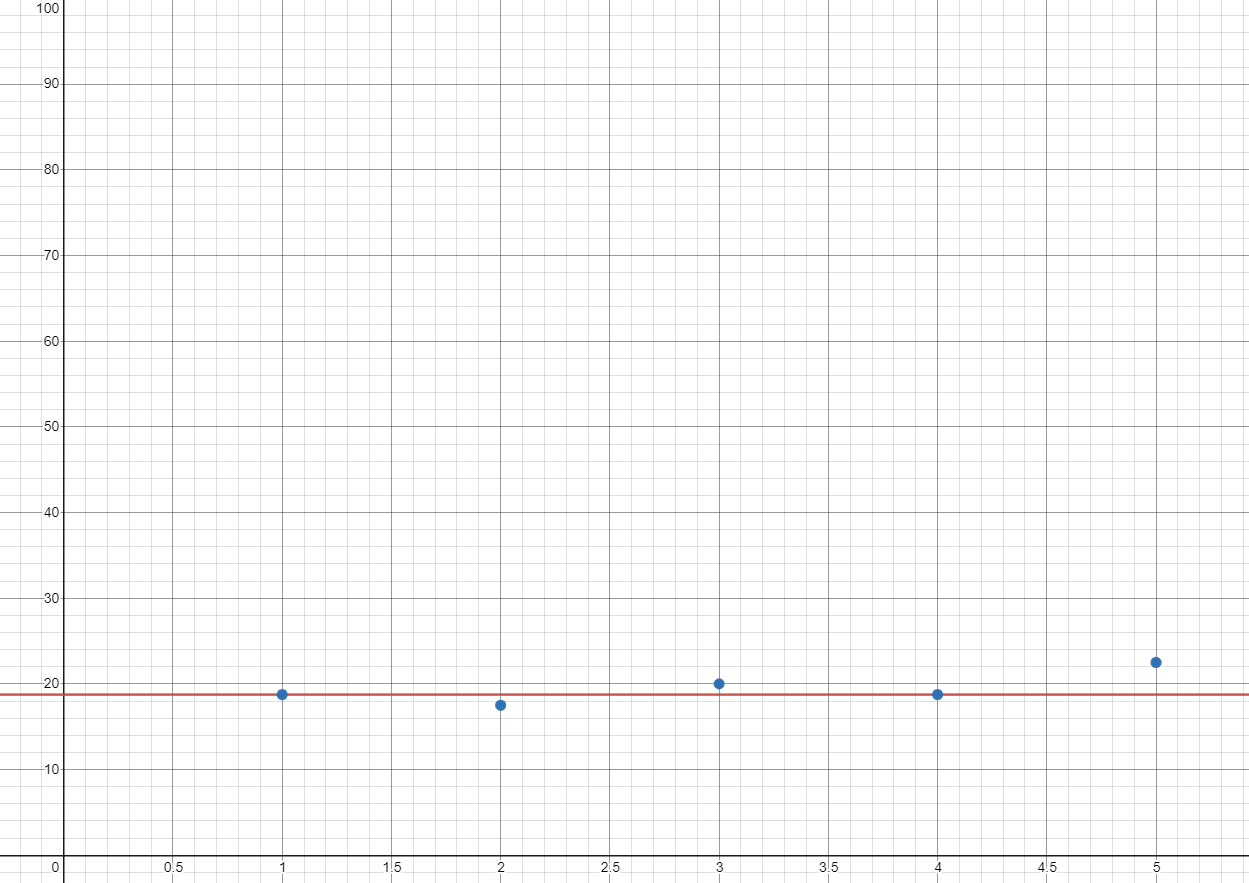
\includegraphics[scale=0.4]{graph.png}
\end{figure} 
x axis is the T value and the y axis is the error rate in percentage

\end{document}










